\documentclass[letterpaper, 10 pt, conference]{ieeeconf} 
\overrideIEEEmargins 
\IEEEoverridecommandlockouts 


%\usepackage[backend=biber,dateabbrev=true,style=ieee]{biblatex}
\usepackage[style=ieee]{biblatex}

\usepackage{acronym}
\usepackage{algorithm}
\usepackage{algpseudocode} % From 5.1 in http://tug.ctan.org/macros/latex/contrib/algorithmicx/algorithmicx.pdf
\usepackage{amsfonts}
\usepackage{amsmath}
\usepackage{amssymb}
\let\proof\relax
\let\endproof\relax
\usepackage{amsthm}
\usepackage{array}
\usepackage{bm}
\usepackage{calc} % For widthof
\usepackage{caption}
\usepackage{environ}         % provides \BODY
\usepackage{etoolbox}        % provides \ifdimcomp
\usepackage{fontawesome}
\usepackage{graphicx}        % provides \resizebox
\usepackage{hyperref}
\usepackage{pgf}
\usepackage{pgfplots}
\usepackage{pifont}
\usepackage{subcaption}
\usepackage{xparse}

\usepackage[T1]{fontenc}
%\bibliographystyle{IEEEtran}
\bibliography{./bib/IEEEabrv,./bib/bibliography}
%\bibliography{./bib/bibliography}
% ========================== Basic ==========================
\newcommand{\dyn}[1]{\ensuremath{#1^x}}        % Related to system dynamics
\newcommand{\dst}[1]{\ensuremath{#1^\sigma}}   % Related to system disturbance 
\newcommand{\st}{\ensuremath{\text{s.t.}}}
% =========================== Sets ==========================
\renewcommand{\int}{\ensuremath{\mathbb{Z}}}
\newcommand{\real}{\ensuremath{\mathbb{R}}}
\newcommand{\nat}{\ensuremath{\mathbb{N}}}
\newcommand{\cset}{\ensuremath{\mathcal{C}}}
\NewDocumentCommand{\idxset}{m}{\ensuremath{\mathcal{I}_{#1}}}
\NewDocumentCommand{\PowerSet}{m}{\ensuremath{\mathcal{P}\left(#1\right)}}
\NewDocumentCommand{\Pre}{ o o m }{%
	\IfNoValueTF{#2}{%
		\IfNoValueTF{#1}{% No #1 or #2
			\ensuremath{\text{Pre}^1\left(#3\right)}
		}{% #1 but no #2
			\ensuremath{\text{Pre}_{#1}^1\left(#3\right)}
		}}{% #1 and #2
			\ensuremath{\text{Pre}^{#2}_{#1}\left(#3\right)}
		}}
%\NewDocumentCommand{\PreviewedPre}{ o o m }{%
%	\IfNoValueTF{#2}{%
%		\IfNoValueTF{#1}{% No #1 or #2
%			\ensuremath{\text{Pre}^{\text{\tiny\faEye},1\hspace{-0.1cm}}\left(#3\right)}
%		}{% #1 but no #2
%			\ensuremath{\text{Pre}_{#1}^{\text{\tiny\faEye},1\hspace{-0.1cm}}\left(#3\right)}
%		}}{% #1 and #2
%			\ensuremath{\text{Pre}^{\text{\tiny\faEye}, #2\hspace{-0.1cm}}_{#1}\left(#3\right)}
%		}}
\NewDocumentCommand{\PreviewedPre}{ o o m }{%
	\IfNoValueTF{#2}{%
		\IfNoValueTF{#1}{% No #1 or #2
			\ensuremath{\text{Pre}^{1\hspace{-0.1cm}}\left(#3\right)}
		}{% #1 but no #2
			\ensuremath{\text{Pre}_{#1}^{1\hspace{-0.1cm}}\left(#3\right)}
		}}{% #1 and #2
			\ensuremath{\text{Pre}^{#2\hspace{-0.1cm}}_{#1}\left(#3\right)}
		}}		
			
% ========================== Ranges =========================
\newcommand{\rgeq}[1]{\ensuremath{_{\geq #1}}}
\newcommand{\rleq}[1]{\ensuremath{_{\leq #1}}}
\newcommand{\rg}[1]{\ensuremath{_{>#1}}}
\newcommand{\rl}[1]{\ensuremath{_{<#1}}}
\newcommand{\rii}[2]{\ensuremath{_{[#1,#2]}}}
\newcommand{\rie}[2]{\ensuremath{_{[#1,#2)}}}
\newcommand{\rei}[2]{\ensuremath{_{(#1,#2]}}}
\newcommand{\ree}[2]{\ensuremath{_{(#1,#2)}}}
\newcommand{\elrii}[2]{\ensuremath{_{\{#1,#2\}}}}

% ===================== Constraint sets =====================
% \_con ----- Produces the constraint set for the indicated quantity. One optional arg adds a substcript.
\NewDocumentCommand{\xcon}{ o o }{%
	\IfNoValueTF{#2}%
	{		
	\IfNoValueTF{#1}%
		{\ensuremath{\mathcal{X}}}%
		{\ensuremath{\mathcal{X}_{#1}}}}
		{\ensuremath{\mathcal{X}{(#1,#2)}}}}
\NewDocumentCommand{\ucon}{ o }{%
	\IfNoValueTF{#1}%
		{\ensuremath{\mathcal{U}}}%
		{\ensuremath{\mathcal{U}_{#1}}}}
\NewDocumentCommand{\tcon}{ o }{%
	\IfNoValueTF{#1}%
		{\ensuremath{\mathcal{T}}}%
		{\ensuremath{\mathcal{T}_{#1}}}}
\NewDocumentCommand{\wcon}{ o o }{%
	\IfNoValueTF{#2}%
		{
		\IfNoValueTF{#1}
			{%
			\ensuremath{\mathcal{W}}%
			}{
			\ensuremath{\mathcal{W}_{#1}}
			}
		}{
		\ensuremath{\mathcal{W}_{#2}^{#1}}
		}}
\NewDocumentCommand{\wconset}{ m }{\ensuremath{\mathcal{W}^{#1}}}

% ==================== Switching signals ====================
% \ss --------- General switching signal
% \sucset ----- Successor matrix associated with signal #1. Ex. \sucmat{\dyn\ss}
% \sucsetel --- Successor matrix element (#2,#3) associated with signal #1. Ex. \sucset{\dyn\ss}{\dyn\modeidx_i}{\dyn\modeidx_j}

% \mindts ----- Vector of the mode-dependent min-DTs for signal #1. Ex \mindts{\dst\ss}
% \maxdts ----- Vector of the mode-dependent max-DTs for signal #1. Ex \maxdts{\dst\ss}
% \mindt ------ The mode-dependent min-DT for signal #1, mode #2. Ex \mindt{\dst\ss}{\dst\modeidx}
% \maxdt ------ The mode-dependent max-DT for signal #1, mode #2. Ex \maxdt{\dst\ss}{\dst\modeidx}
% \sucsetcon -- Succesoor matrix constraint

% \mindtscon -- Vector of min-dt constraints
% \maxdtscon -- Vector of max-dt constraints
% \mindtcon --- Single min-dt constraint
% \maxdtcon --- Single max-dt constraint
% \ssset     -- Set of switching signals that respects up to three constraint elements

% \sstimer   -- Ss timer. Maps the time and a ss to the number of steps since a switch that new information was gleaned
% \sstimerval - A Value of switching signal timer
% \sstimermax - Maximum value of the switching signal timer in mode #1
% \sspairset -- The set of possible pairs given a mode #1 and timer value #2
% \sscount ---- The number of times the switching signal has changed at some time t

\renewcommand{\ss}{\ensuremath{{\sigma}}}
\newcommand{\ssg}{\ensuremath{{\sigma^\mathcal{G}\text{\hspace{0pt-\widthof{$^\mathcal{G}$}}}}}}
\NewDocumentCommand{\ssl}{o}{%
	\IfNoValueTF{#1}{
		\ensuremath{{\sigma^\mathcal{L}}}
		}{
		\ensuremath{{\sigma^\mathcal{L}_{#1}}}}}
\newcommand{\sucset}[1]{\ensuremath{\mathcal{S}^{#1}}}
\newcommand{\sucsetrow}[2]{\ensuremath{\sucset{#1}_{#2}}}
\newcommand{\sucsetel}[3]{\ensuremath{{s_{#2,#3}^{#1}}}}

\newcommand{\mindts}[1]{\ensuremath{\underline{\mathcal{D}}^{#1}}}
\newcommand{\maxdts}[1]{\ensuremath{\overline{\mathcal{D}}^{#1}}}
\newcommand{\mindt}[2]{\ensuremath{{\underline{\delta}_{#2}^{#1}}}}
\newcommand{\maxdt}[2]{\ensuremath{{\overline{\delta}_{#2}^{#1}}}}
\newcommand{\sucsetcon}{\ensuremath{{S}}}
\newcommand{\sucsetconrow}[1]{\ensuremath{{S_{#1}}}}

\newcommand{\mindtscon}{\ensuremath{\underline{D}}}
\newcommand{\maxdtscon}{\ensuremath{\overline{D}}}
\newcommand{\mindtcon}[1]{\ensuremath{{\underline{d}_{#1}}}}
\newcommand{\maxdtcon}[1]{\ensuremath{{\overline{d}_{#1}}}}
%\newcommand{\ssset}[3]{\ensuremath{\Sigma(#1,#2,#3)}}
\NewDocumentCommand{\ssset}{ o o o }{%
	\IfNoValueTF{#3}%
		{\IfNoValueTF{#2} %no 3
			{\IfNoValueTF{#1}%no 2, no 3
				{\ensuremath{\Sigma}}
				{\ensuremath{\Sigma(#1)}}
			}
			{\ensuremath{\Sigma(#1,#2)}}%no 3 but 1 and 2
		}
		{\ensuremath{\Sigma(#1,#2,#3)}}}
		
\newcommand{\sstimer}{\ensuremath{{T}}}
\newcommand{\sstimerval}{\ensuremath{\tau}}
%\newcommand{\sstimermax}[1]{\ensuremath{{\overline{\sstimerval}_{#1}}}}
\NewDocumentCommand{\sstimermax}{o m}{%
	\IfNoValueTF{#1}{
		\ensuremath{{\overline{\sstimerval}_{#2}}}
		}{
		\ensuremath{{\overline{\sstimerval}_{#2}^{#1}}}}}
\newcommand{\sspairset}[2]{\ensuremath{{\Lambda((#1,#2))}}}
\newcommand{\sscount}{\ensuremath{{\ss^\#}}}

\newcommand{\switchtimes}[1]{\ensuremath{\tau^{#1}}}
\newcommand{\switchtime}[2]{\ensuremath{{\switchtimes{#1}_{#2}}}}
\newcommand{\lastswitchtime}[1]{\switchtimes{#1}_+}

% ================== System Agents ==================
\newcommand{\agents}{\ensuremath{\mathcal{M}}}
\newcommand{\agent}[1]{\ensuremath{\agents^{#1}}}
\newcommand{\numagents}{\ensuremath{{N_a}}}
\newcommand{\agentidx}{\ensuremath{\alpha}}
\newcommand{\agentidxset}{\ensuremath{\mathcal{I}^a}}

% ================== System Modes ==================
% \modes -------- A collection of modes. May optionally specify parent agent.
% \mode --------- A single mode indexed by #1
% \nummodes --- Number of modes 
% \modeidx ------ Index of a single mode \ss(t)=\modeidx

% \ ------------- The state dimension
% \nu ------------- The input dimension

\NewDocumentCommand{\modes}{o}{%
	\IfNoValueTF{#1}{
		\ensuremath{\mathcal{M}}
		}{
		\ensuremath{\mathcal{M}^{#1}}}}
\NewDocumentCommand{\mode}{o m}{%
	\IfNoValueTF{#1}{
		\ensuremath{\modes_{#2}}
		}{
		\ensuremath{\modes[#1]_{#2}}}}
\NewDocumentCommand{\nummodes}{o}{%
	\IfNoValueTF{#1}{
		\ensuremath{|\modes|}
		}{
		\ensuremath{{|\modes^{#1}|}}}}
\newcommand{\modeidx}{{\ensuremath{\mu}}}
\NewDocumentCommand{\modeidxset}{o}{%
	\IfNoValueTF{#1}{
		\ensuremath{\ensuremath{\mathcal{I}^m}}
		}{
		\ensuremath{\ensuremath{\mathcal{I}_{#1}^m}}}}
\newcommand{\nx}{\ensuremath{{n_x}}}
\renewcommand{\nu}{\ensuremath{{n_u}}}
\newcommand{\nw}{\ensuremath{{n_w}}}
\NewDocumentCommand{\futstate}{ o o o o}{%
	\IfNoValueTF{#3}%
		{\ensuremath{x{(#1,#2)}}}
		{\ensuremath{\phi(#1;#2,#3,#4)}}}
\NewDocumentCommand{\useq}{}{\ensuremath{\mathfrak{u}}}
\NewDocumentCommand{\feasuseq}{mmm}{%
	\ensuremath{\mathfrak{U}(#1,#2,#3)}
	}
	
	
% ==================== Safe sets ====================
\newcommand{\safesets}{\ensuremath{\mathcal{S}}}
\newcommand{\safeset}[1]{\ensuremath{\safesets_{#1}}}

% ==================== Misc ====================
\newcommand{\narroweq}{\ensuremath{\scalerel[1ex]{=}{\phantom{=}\hspace{-0.17cm}}}}

% ============== Autoref Titles ================
\renewcommand{\equationautorefname}{Equation}
\renewcommand{\sectionautorefname}{Section}
\newcommand{\remarkautorefname}{Remark}
\newcommand{\algorithmautorefname}{Algorithm}

% ============== Directed Graph ================
\NewDocumentCommand{\graph}{}{\ensuremath{\mathcal{G}}}
\NewDocumentCommand{\gnumnodes}{o}{
	\IfNoValueTF{#1}
		{\ensuremath{|\graph|}}
		{\ensuremath{|\graph^{#1}|}}}
\NewDocumentCommand{\gedges}{}{\ensuremath{\mathcal{E}}}
\NewDocumentCommand{\gnodeedges}{o m}{
	\IfNoValueTF{#1}
		{\ensuremath{\gedges_{#2}}}
		{\ensuremath{\gedges_{#2}^{#1}}}}
\NewDocumentCommand{\glabels}{}{\ensuremath{\mathcal{L}}}
\NewDocumentCommand{\gnodelabel}{m}{\ensuremath{\glabels_{#1}}}
\NewDocumentCommand{\gnumlabels}{}{\ensuremath{\overline{\graph}}}
\newacro{mpc}[MPC]{model predictive control}
\newacro{mindt}[min-DT]{minimum dwell time}
\newacro{maxdt}[max-DT]{maximum dwell time}
\newacro{pi}[PI]{positive invariant}
\newacro{ci}[CI]{Control invariant}

\newtheorem{theorem}{\textbf{Theorem}}
\newtheorem{lemma}{\textbf{Lemma}}
\newtheorem{corollary}{\textbf{Corollary}}
\newtheorem{definition}{Definition}
\newtheorem{assumption}{Assumption}
\theoremstyle{remark}
\newtheorem*{remark}{Remark}
\newtheorem{case}{Case}
\newtheorem{problem}{Problem}

\newcommand{\alert}[1]{\textbf{\color{red}{\MakeUppercase{#1}}\color{black}}}

\renewcommand{\theoremautorefname}{Theorem}
\renewcommand{\algorithmautorefname}{Algorithm}
\newcommand{\definitionautorefname}{Def.}
\newcommand{\lemmaautorefname}{Lemma}
\newcommand{\assumptionautorefname}{Assumption}

% For do-while algorithm loops (https://tex.stackexchange.com/questions/115709/do-while-loop-in-pseudo-code)
\algdef{SE}[DOWHILE]{Do}{doWhile}{\algorithmicdo}[1]{\algorithmicwhile\ #1}%
\renewcommand{\algorithmicrequire}{\textbf{Input:}}
\renewcommand{\algorithmicensure}{\textbf{Output:}}
% declaration of the new block
\algblock{ParFor}{EndParFor}
% customising the new block
\algnewcommand\algorithmicparfor{\textbf{parfor}}
\algnewcommand\algorithmicpardo{\textbf{do}}
\algnewcommand\algorithmicendparfor{\textbf{end\ parfor}}
\algrenewtext{ParFor}[1]{\algorithmicparfor\ #1\ \algorithmicpardo}
\algrenewtext{EndParFor}{\algorithmicendparfor}


%\NewDocumentCommand{\edit}{m m}{#2}
\NewDocumentCommand{\edit}{m m}{{\color{red}#1 }{\color{blue}#2}}

\newlength{\myl}
\let\origequation=\equation
\let\origendequation=\endequation
\RenewEnviron{equation}{
  \settowidth{\myl}{$\BODY$}                       % calculate width and save as \myl
  \origequation
  \ifdimcomp{\the\linewidth}{>}{\the\myl}
  {\ensuremath{\BODY}}                             % True
  {\resizebox{\linewidth}{!}{\ensuremath{\BODY}}}  % False
  \origendequation
}

\pgfplotsset{compat=1.17}
\pdfminorversion=4

\def\BibTeX{{\rm B\kern-.05em{\sc i\kern-.025em b}\kern-.08em T\kern-.1667em\lower.7ex\hbox{E}\kern-.125emX}}

\title{\LARGE \bf Parallelized Algorithm for Persistent Feasibility in Linear Systems with Multiple, External Switching Signals}
\author{Richard A Hall$^{1}$ and Dr. Leila Bridgeman$^{2}$% <-this % stops a space
\thanks{$^{1}$Richard A Hall is a Ph.D student in the Thomas Lord MEMS Department, Duke University, Durham NC, USA
        {\tt\small rah75@duke.edu}}%
\thanks{$^{2}$Leila Bridgeman is an associate professor with the the Thomas Lord MEMS Department, Duke University, Durham NC, USA {\tt\small leila.bridgeman@duke.edu}}%
}

\begin{document}
\maketitle
\thispagestyle{empty}
\pagestyle{empty}
%\author{\IEEEauthorblockN{1\textsuperscript{st} Richard A Hall}
%\IEEEauthorblockA{\textit{Thomas Lord MEMS Department} \\
%\textit{Duke University}\\
%Durham, NC, USA \\
%0000-0003-3512-6941}
%\and
%\IEEEauthorblockN{2\textsuperscript{nd} Leila Bridgeman}
%\IEEEauthorblockA{\textit{Thomas Lord MEMS Department} \\
%\textit{Duke University}\\
%Durham, NC, USA \\
%0000-0002-9367-7218}
%}
%\maketitle
\begin{abstract}
Ensuring feasibility in externally switched systems usually requires identifying time-varying, control invariant (CI) sets that ensure state and input constraints can be respected under any possible switching signal. As with traditional, time-invariant CI sets, these time-varying constraints can be very difficult to compute for higher dimensional systems. Furthermore, if multiple switching signals are present, the number of possible permutations of these signal values grows exponentially. Previous works would struggle to account for this growth. Inspired by distributed systems, this work examines a class of high dimensional systems with multiple switching signals. The switching signals are constrained using directed graphs that are significantly more flexible than dwell time based methods used in much of the previous literature. An iterative algorithm is developed that computes the time-varying CI sets for this class of systems. Critically, this algorithm is parallelized over the number of agents, preventing the exponential growth in computation time as agents are added to the system. The scalability of the results results is demonstrated on a randomized numerical example.
\end{abstract}
\section{Introduction}
Hybrid systems are a broad and important class of systems with both discrete and continuous (or discrete approximations of continuous) dynamics. A subclass of these are systems whose discrete dynamics are purely time dependent and unknown to the system. For example, user input and component failures can both cause the system to suddenly change. Such discrete, external dynamics can be viewed as an external signal switching the system's dynamics at discrete, unforeseen times. If the system is constrained, then special care should be taken to make the system robust to these switches so that constraints are not violated. 

If the system were allowed to be switched arbitrarily, then satisfying the constraints would require the controller to always keep the state within a control invariant set common to all modes \cite{Liberzon1999}. If the modes are not extremely similar, this may be a very difficult or impossible requirement meet. Instead of arbitrary switching, dwell time and successor constraints are often imposed on the switching signal \cite{Liberzon1999,Morse1999}. Minimum dwell time constraints give the system time to recover after a switch and prepare for the next one \cite{Danielson2019}, while maximum dwell time constraints ensure that the system will not dwell in ``poorly'' behaved modes for too long \cite{Hall2022}. These constraints can either be generated by the physical implementation and the controller designed to accommodate them (as in \cite{Danielson2019}), or they can be specified by the controller and enforced in the physical implementation (as in \cite{Zhang2016}). Dwell time and successor constraints have been used in previous works to create time-varying control invariant sets that are robust to all possible switching signals \cite{Danielson2019}. Unfortunately, these methods can be very computationally expensive and suffer greatly from the curse of dimensionality, precluding their use in large-scale systems and motivating the techniques developed here.

A further shortcoming of the current literature is that only a single switching signal is explicitly considered. A naive solution to this would simply be to define a new switching signal with states corresponding to all the realizable permutations of the independent signals. While this would work in theory, it creates an exponential growth in the number of possible signal states. Seeking to enumerate these with even just two switching signals and define the dwell time and successor constraints of each mode quickly leads back to arbitrary switching and its associated challenges. Even if some weaker constraints could be maintained, the increase in the computational load with be difficult to overcome.

This work develops an algorithm with applications to both reduce the computational expense of previous algorithms and analyze of systems with multiple sources of switching. The algorithm's most computationally expensive steps are parallelizable, greatly improving its scalability. In the next section, notation and concepts are introduced that will be used throughout the reminder of the paper. Next, the general form of the system is described and the associated challenges are discussed further. Finally, several algorithms are introduced as key contributions of this work and their theoretical properties and implementation are explored. These are then applied to a numerical example that demonstrates their effectiveness. 

Related works includes \cite{Ahandani2020} where the authors examine decentralized systems under MPC with switching communication topologies and coupling in the constraints and inputs. The local agents are assumed LTI while the cross dynamics change according to the switching signal. This leads to an external disturbance applied to each node that is rejected using tube-based, switched MPC.
% \section{Literature Review}
 \subsection{Key contributions of this paper}
 This paper examines systems that
 \begin{enumerate}
 	\item are distributed,
 	\item are coupled through states,
 	\item are uncoupled through constraints,
 	\item have locally switching dynamics,
 	\item have a switching network according to local switches,
 	\item have local, constrained, external switching signals.
 \end{enumerate}
 How does this compare with other papers?

\cite{Ahandani2020} examines decentralized systems under MPC with switching communication topologies and dynamics coupling. The switching is generated from a centralized signal with a minimum dwell time constraint. The local agents are assumed LTI while the cross dynamics change according to the switching signal. This leads to an external disturbance drawn from a switching set applied to each node. This is rejected using tube-based, switched MPC. 

\cite{Monasterios2019} examines systems under MPC that are provided a preview of future disturbances. The preview evolves through disturbed shifting dynamics. The primary results of the paper show that, if the change in disturbance is ``small enough'', the system can maintain feasibility and stability with augmented terminal control elements. It does not, however, consider switching either locally nor remotely. 
 
%%\begin{center}
\renewcommand{\arraystretch}{1.5}
\begin{table}[t]
\begin{tabular}{|m{1cm}|m{6.8cm}|}
\hline
\textbf{Symbol} & \textbf{Description}\\
\hline\hline
$\numagents$ & Number of switching signals/agents\\
\hline
$\agentidxset$ & Set of agent indicies, $\int\rii{1}{\numagents}$\\
\hline
$\nummodes[\agentidx]$ & Number of modes in agent $\agentidx\in\agentidxset$\\
\hline
$\modeidxset[\agentidx]$ & Set of mode indicies in agent $\agentidx$, $\int\rii{1}{\nummodes[\agentidx]}$\\
\hline
\end{tabular}
\end{table}
\end{center}
\section{Preliminaries}
\subsection{Notation}
Let $\mathcal{S}=\{\{\{\mathcal{S}_{(i,j,k)}\}_{k\in\mathcal{I}_{K}(i,j)}\}_{j\in\mathcal{I}_{J}(i)}\}_{i\in\mathcal{I}_I}$, $\mathcal{S}\subseteq\real^n$ be a nested collection of subsets of the $n$-dimensional, real-valued numbers. The first and second level sub-collections are denoted as $\mathcal{S}_{(i)}=\{\{\mathcal{S}_{(i,j,k)}\}_{k\in\mathcal{I}_{K}(i,j)}\}_{j\in\mathcal{I}_{J}(i)}$ and $\mathcal{S}_{(i,j)}=\{\mathcal{S}_{(i,j,k)}\}_{k\in\mathcal{I}_{K}(i,j)}$. Operations preformed between nested collections require the collections be of equal size and are preformed elementwise. For example, $\mathcal{S}_{(i)}$ equals $\tilde{\mathcal{S}}_{(i)}$ if they are the same size and every element in both are equivalent. Operations preformed between a nested collection and a single element behave as if the single element where an appropriate sized collection with elements equal to the single element. For example, setting $\mathcal{S}=\underline{0}$ sets every element of $\mathcal{S}$ to $\underline{0}$. Finally, union operations are preformed on every element of the nested collection. For example, $\cup \mathcal{S}_{(i)}$ is the union of all the elements of $\mathcal{S}_{(i)}$.

\subsection{Set Operations}
Set operations provide tools to analyze how a system can evolve under allowable inputs. Given a disturbed linear system with state and input constraints, $\mode{\modeidx}\triangleq\{A_\modeidx, B_\modeidx, E_\modeidx,\xcon[\modeidx],\ucon[\modeidx]\}$ where $x(t+1)=A_\modeidx x(t)+ B_\modeidx u(t)+ E_\modeidx w(t)$, the following important set operations are introduced. 
\begin{definition}[Robust Preset]
The $k$-step, robust preset of a set $\mathcal{S}$ under the constrained dynamics $\mode{\modeidx}$ and disturbance $w\in\wcon$ is given by
\begin{align}
\Pre[\modeidx][0]{\mathcal{S},\wcon}&\triangleq\mathcal{S},\\
\Pre[\modeidx][k]{\mathcal{S},\wcon}&\triangleq\{x\in\xcon\ |\ \exists u\in\ucon\text{ s.t. }\forall w\in\wcon,\nonumber\\ &A_\modeidx x+ B_\modeidx u+ E_\modeidx w\in\Pre[\modeidx][k-1]{\mathcal{S},\wcon}\}.
\end{align}
\end{definition}
\begin{definition}[Previewed Robust Preset]
The $k$-step, previewed robust preset of a set $\mathcal{S}$ under the constrained dynamics $\mode{\modeidx}$ and disturbance $w\in\wcon$ is given by
\begin{align}
\PreviewedPre[\modeidx][0]{\mathcal{S},\wcon}&\triangleq\mathcal{S},\\
\PreviewedPre[\modeidx][k]{\mathcal{S},\wcon}&\triangleq\{x\in\mathcal{X}|\forall w\in\mathcal{W},\exists u\in\mathcal{U}\text{ s.t. }\nonumber\\
&A_\modeidx x+ B_\modeidx u+ E_\modeidx w\in\PreviewedPre[\modeidx][k-1]{\mathcal{S},\wcon}\}.
\end{align}
\end{definition}
The previewed robust preset is a superset or equal to the standard robust presets.  They can be found using basic set operation such as the Minkowski sum and difference as shown below \cite{Borrelli2017}.
\begin{align}
\Pre[][1]{\mathcal{S}} &= \left(\left(\left(\mathcal{S}\ominus A_w\circ\mathcal{W}\right)\oplus\left(-B\circ\mathcal{U}\right)\right)\circ A\right)\ \cap\ \mathcal{X},\\
\PreviewedPre[][1]{\mathcal{S}} &= \left(\left(\left(\mathcal{S}\oplus\left(-B\circ\mathcal{U}\right)\right)\ominus A_w\circ\mathcal{W}\right)\circ A\right)\ \cap\ \mathcal{X}.
\end{align}

\subsection{Feasibility Analysis}
In constrained systems, it is critically important that the controller can satisfy the state constraints using only feasibly inputs. If a feasible input exists such that the resulting state is also feasible, the system is feasible. If feasibility at the current time implies feasibility at all future times, then the system is persistently feasible.

One way to ensure persistent feasibility is by constraining the system to be within a control invariant set that is a subset of the state constraints. Since the definition of control invariance implies that a feasible input exists that will keep the system in the set if it starts in the set, then at least this single input, and possibly others, can serve as a feasible input. This will continue for all time establishing persistent feasibility. 

Relying on constant, control invariant sets become difficult in externally switched systems, however. The set must be common to all system modes are persistent feasibility is lost. This concern can be addressed using time varying, control invariant sets that take advantage of constraints on the switching signal. For example, in \cite{Danielson2019,Santis2004}, time varying, control invariant sets where developed that force the system to move during the minimum dwell time to a region that will be safe for any successor mode.

The ideas presented in the previous literature can be described using the concepts of safe-set collections. These are collections of sets, indexed by some time varying signal, that serve as the active state constraints of the system. To establish persistent feasibility, they require that every set is witching the 1-step preset of all possible successor sets. This is presented formally in the following definition.
\begin{definition}[Safe-set collection]
Let $\ss:\int\rgeq 0\rightarrow \{1,...,\nummodes\}$ be an external signal that selects the current mode of $\mode{}(t)=\{f_{\ss(t)}(x(t),u(t)),\xcon[\ss(t)],\ucon[\ss(t)]\}$ and let $\ss^+$

 a collection of sets, $\mathcal{S}=\{\mathcal{S}_{i_1},...,\mathcal{S}_{i_N}\}$ is a safe-set collection if there exists a mapping between time and the current mode index, $g:\int\rgeq{0}\rightarrow\{i_1,...,i_N\}$ and another mapping between the current time and possible  indicies at the next step, $g^+:\int\rgeq 0\rightarrow\mathcal{P}(\{i_1,...,i_N\})$ such that
$$\mathcal{S}_{g(t-1)}\subseteq\Pre[\mode{}(t)][1]{\mathcal{S}_{g(t)}}\ \forall\ g(t)\in g^+(t-1)$$
\end{definition}

%\begin{figure*}[t]
%\centering
%\includegraphics[width=\textwidth]{./figures/sample_system}
%\end{figure*}

\section{System Description}
In the previous \edit{sections}{section}, the systems have only contained a single switching signal. In general, however, switching signals may come from independent sources and merging them into a single signal would \edit{be less}{not be} justified. 

\edit{Consider a collection of $\numagents\in\int\rgeq{1}$ external switching signals each respecting their own directed graph, $\ss_\agentidx(t)\in\Sigma(\graph^\agentidx)\ \agentidx\in\idxset{\numagents}$. Further, consider a system with all of these signals and dynamics taking the form}{Consider a linear system partitioned into $\numagents$ agents where agent $\agentidx\in\idxset{\numagents}$ has states $x_\agentidx(\cdot)\in\real^{n_x^\alpha}$ and inputs $u_\agentidx(\cdot)\in\real^{n_u^\alpha}$. Each agent switches according to the local switching signal, $\ss_\agentidx(t)\in\Sigma(\graph^\agentidx),\ \agentidx\in\idxset{\numagents}$. These dynamics can be represented centrally as}
\begin{subequations}
\label{eq:sys}
\begin{align}
A(t)&=\begin{bmatrix}
A^{11}_{\ssl[1](t)}&A^{12}_{\ssl[1](t)}&\cdots&A^{1\numagents}_{\ssl[1](t)},\\
A^{21}_{\ssl[2](t)}&A^{22}_{\ssl[2](t)}&\cdots&A^{2\numagents}_{\ssl[2](t)},\\
\vdots&\vdots & \ddots & \vdots\\
A^{\numagents 1}_{\ssl[\numagents](t)} & A^{\numagents 2}_{\ssl[\numagents](t)} &\cdots & A^{\numagents \numagents}_{\ssl[\numagents](t)} 
\end{bmatrix},\label{eq:sys_A}\\
B(t)&=\begin{bmatrix}
B^{1}_{\ssl[1](t)} & \cdots & 0\\
\vdots             & \ddots & \vdots\\
0                  & \cdots & B^{\numagents}_{\ssl[\numagents](t)}
\end{bmatrix},\label{eq:sys_B}\\
\xcon(t)&=\xcon[\ssl[1](t)]^1\times\cdots\times\xcon[\ssl[\numagents](t)]^\numagents,\label{eq:sys_X}\\
\ucon(t)&=\ucon[\ssl[1](t)]^1\times\cdots\times\ucon[\ssl[\numagents](t)]^\numagents\label{eq:sys_Y}.
\end{align}
\end{subequations}
This structure is motivated by distributed systems with coupling in the system's states. Note how each block-row is governed by a single switching signal. This makes intuitive sense because local switching signals are more likely to effect how neighboring states impact the local agent rather then how local states will effect neighboring agents.

The goal of this work is to design a safe-set collection for systems with the above structure. \edit{A single signal could amalgamate all the individual switching signals. The definition of safe-sets, however, clearly shows that the exponential growth in the number of graph nodes corresponds to is an exponential growth in the cardinality of the safe-set collection.}{One possible solution could be to amalgamate the individual switching signals into a single signal and treat the system as centralized. This would cast the problem in the form of \autoref{eq:basic_switched_sys} and previous results could be used to compute a safe-set collection for the system \cite{Danielson2019}. However, this would lead to exponential growth in the number of nodes in the switching signal's graph matched by growth in the elements of the safe-set collection.}  This is computationally untenable. This is further exasperated in the high dimension systems with the block-row structure would tend to have. Having even just three block-rows each in $\real^3$ leads to a nine-dimensional system and will tax this naive implementation. These concerns will be addressed by splitting the system into block-rows and looking for safe-set collections, $\mathcal{S}^{\agentidx}=\{\mathcal{S}^\agentidx_n\}_{n\in\gnumnodes[\agentidx]}$, for each separately. Once found, the collections can be merged into a large collection with all possible switching signal states represented.

Looking only at the block row indexed by $\agentidx$, the dynamics can be rewritten as 
\edit{
\begin{align}
x_\agentidx(t+1)&=A^{\agentidx\agentidx}_{\ssl[\agentidx](t)}x_\agentidx(t)+B^\agentidx_{\ssl[\agentidx](t)}u_\agentidx(t)\nonumber\\&\quad+\sum_{\tilde\agentidx\in\idxset{\numagents}\setminus \agentidx}A^{\agentidx\tilde\agentidx}_{\ssl[\agentidx](t)}x_{\tilde\agentidx}(t)\\
&=A^{\agentidx}_{\ssl[\agentidx](t)}x_\agentidx(t)+B^\agentidx_{\ssl[\agentidx](t)}u_\agentidx(t)+E_{\ssl[\agentidx](t)}^\agentidx w(t),\nonumber
\end{align}
with $w(t)\in\wcon[\ssl[\agentidx](t)]^\agentidx$.}{\begin{align}\label{eq:block-row-dyn}
x_\agentidx(t+1)&=A^{\agentidx}_{\ssl[\agentidx](t)}x_\agentidx(t)+B^\agentidx_{\ssl[\agentidx](t)}u_\agentidx(t)+E_{\ssl[\agentidx](t)}^\agentidx w(t)
\end{align}
where
\begin{align*}
E_{\ssl[\agentidx](t)}^\agentidx =\left[A^{\agentidx\tilde\agentidx}_{\ssl[\agentidx](t)}\right]_{\tilde\agentidx\in\idxset{\numagents}\setminus \agentidx}\in\real^{n_x^\agentidx \times \sum_{\tilde\agentidx\in\idxset{\numagents}\setminus \agentidx} n_x^{\tilde\agentidx}}
\end{align*}
and $w(t)\in\wcon[\ssl[\agentidx](t)]^\agentidx\subset \real^{ \sum_{\tilde\agentidx\in\idxset{\numagents}\setminus \agentidx} n_x^{\tilde\agentidx}}$.}
 The existence of $\wcon[\ssl[\agentidx](t)]^\agentidx$ can be inferred from the fact that the full system is constrained. These dynamics and constraints are collected into the following tuple defining agent $\agentidx$,
$$\agent{\agentidx}\triangleq\{\{A^{\agentidx}_{\modeidx},B^\agentidx_{\modeidx}, E_{\modeidx}^\agentidx,\xcon[\modeidx]^\agentidx,\ucon[\modeidx]^\agentidx, \wcon[\modeidx]^\agentidx\}_{\modeidx=1}^{\nummodes[\agentidx]},\graph^\agentidx\}.$$
These can be collected into the full system
\begin{equation}\label{eq:agent_notation}
\agents\triangleq\{\agent{\agentidx}\}_{\agentidx\in\idxset{\numagents}}.
\end{equation}
Each agent only has a single switching signal explicitly appearing, $\ss_\agentidx(t)$, and resembles a locally switched system with additive disturbances. Previous, robust switched techniques, such as those developed in \cite{Lavaei2021}, may seem like possible solutions. However, $\wcon[\modeidx]^\agentidx$ is unknown. Though it can be characterized using the full state constraints, this would lead to conservative results because the actual safe-sets are, by definition, subsets of the state constraints. Alternatively, each of the neighboring agents could share its current safe-set. This however, returns the system to the centralized problem with its associated drawbacks. Furthermore, if \autoref{eq:block-row-dyn} represents a distributed system, this level of communication may be undesirable. Balancing these considerations, this work bounds the states of any given neighbor within the convex hull of the union of that neighbor's safe-set collection. This only requires acquiring a single set and relies on the state of the local switching signal alone. 
\section{Algorithm Design}
We begin with an algorithm to find the safe-sets of a single agent, $\agent{\agentidx}$, assuming the the other agents' safe-sets are fixed. Let $\mathcal{W}_{\tilde{\agentidx}}$, $\tilde{\agentidx}\in\int\rii{1}{\numagents}\setminus\agentidx$ be the convex hull of the union of the safe-sets for each of the other agents and define 
\begin{equation}
\wcon[\agentidx][\modeidx]=\bigoplus_{\tilde{\agentidx}\in\int\rii{1}{\numagents}\setminus\agentidx}A_\modeidx^{\agentidx,\tilde{\agentidx}}\mathcal{W}_{\tilde{\agentidx}}.
\end{equation}
This represents the set of additive errors agent $\agent{\agentidx}$ can experience while in mode $\modeidx$. Denote the collection of these sets as $\wconset{\agentidx}=\{\wcon[\agentidx][\modeidx]\}_{\modeidx=1}^{\nummodes[\agentidx]}$. With these definitions, the following algorithm is introduced. 
\begin{algorithm}[t]
\caption{Nodal safe-sets with previewed disturbances}\label{alg:node_safe_sets}
\begin{algorithmic}[1]
\Procedure {NodalSafeSets}{$\agent{\agentidx}$, $\wcon$}
\State $k\gets0$
\State $\Omega_{(\modeidx,\sstimerval)}^k\gets\xcon[\modeidx]$ for all $\modeidx\in\int\rii{1}{\nummodes[\agentidx]},\ \sstimerval\in\int\rii{1}{\sstimermax{\modeidx}}$.
\Repeat 
	\State $k\gets k+1$
	\For{$\modeidx\in\int\rii{1}{\nummodes[\agentidx]}$}
		\For{$\sstimerval\in\int\rii{1}{\sstimermax{\modeidx}}$}
			\State $\Omega_{(\modeidx,\sstimerval)}^k\gets\Omega_{(\modeidx,\sstimerval)}^{k-1}$
			\For{$(\tilde{\modeidx},\tilde{\sstimerval})\in\sspairset{\modeidx}{\sstimerval}$}
				\State $\Omega_{(\modeidx,\sstimerval)}^k\gets\Omega_{(\modeidx,\sstimerval)}^k\cap\PreviewedPre[\tilde{\modeidx}][1]{\Omega_{(\tilde{\modeidx},\tilde{\sstimerval})}^{k-1}, \wcon[\agentidx][\modeidx]}$
			\EndFor
		\EndFor
	\EndFor
\Until{$\Omega_{(\modeidx,\sstimerval)}^k=\Omega_{(\modeidx,\sstimerval)}^{k-1}\ \forall\ \modeidx\in\int\rii{1}{\nummodes[\agentidx]},\ \sstimerval\in\int\rii{1}{\sstimermax{\modeidx}}$}
$\safeset{\modeidx}{\sstimerval}\gets\Omega_{(\modeidx,\sstimerval)}^k$ for all $\modeidx\in\int\rii{1}{\nummodes[\agentidx]},\ \sstimerval\in\int\rii{1}{\sstimermax{\modeidx}}$.\;
\EndProcedure
\end{algorithmic}
\end{algorithm}


\begin{algorithm}[t]
\caption{Distributed safe-set collection}\label{alg:safe_sets}
\begin{algorithmic}[1]
\Procedure {SystemSafeSets}{$\agents$}
\State $\Omega^0\gets\{\{\{\underline{0}\}_{\tau\in\mathcal{I}_\tau(\agentidx,\modeidx)}\}_{\modeidx\in\mathcal{I}_\modeidx(\agentidx)}\}_{\agentidx\in\mathcal{I}_\agentidx}$
\State $k\gets0$
\Repeat 
	\State $\Phi^k\gets\{\Call{ConHull}{\bigcup\Omega^k_{(\agentidx)}}\}_{\agentidx\in\mathcal{I}_\agentidx}$
	\For{$\agentidx\in\mathcal{I}_\agentidx$}
		\State $\Omega^{k+1}_{(\agentidx)}\gets\Call{NodeSafeSets}{\modes[\agentidx], \Phi^k}$
	\EndFor
\Until{$\Omega_{(\agentidx)}^k=\Omega_{(\agentidx)}^{k-1}\ \forall\ \agentidx\in\mathcal{I}_\agentidx$}

\State $\safesets\gets\Omega^k$
\EndProcedure
\end{algorithmic}
\end{algorithm}
\section{Numerical Example}
\begin{figure}
	\centering
	\begin{subfigure}[c]{0.475\columnwidth}%
		\centering
		\includegraphics[width=\textwidth]{./figures/num_ex_sys}%
		\caption{Array of linked spring-mass-damper systems. The mass of each object can switch independently according to a directed graph.}%
		\label{fig:num_ex_sys}%
	\end{subfigure}%
	\hfill
	\begin{subfigure}[c]{0.475\columnwidth}%
		\centering
		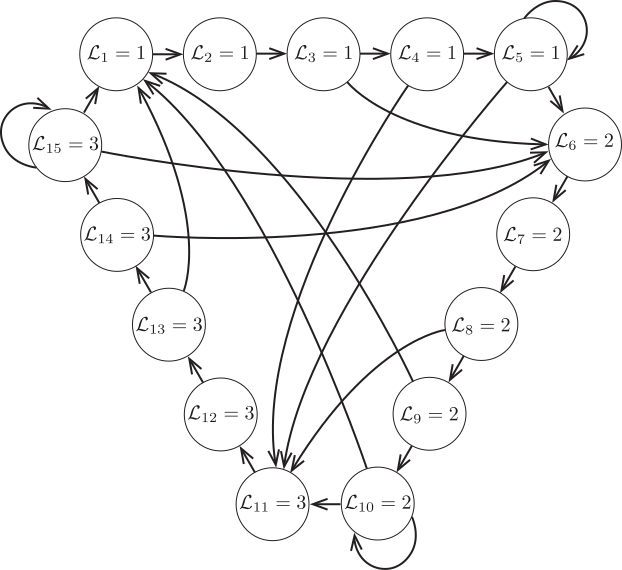
\includegraphics[width=0.8\textwidth]{./figures/num_ex_graph}%
		\caption{Directed graph controlling the switches of the numerical example. Note that the switching constraints cannot be encoded with minimum and maximum dwell times and demonstrate the flexibility of the proposed approach.}%
		\label{fig:num_ex_graph}%
	\end{subfigure}%
	\caption{Description of the system used in the example.}%
\end{figure}

\begin{figure}[t]
\centering
\includegraphics[width=0.9\columnwidth]{./figures/num_ex_results}
\caption{Evolution of the safe-set for a single node of a single agent in the spring-mass-damper array. Though each safe-set shown is feasible, they monotonically increase to convergence with the number of iterations.}
\label{fig:num_ex_results}
\end{figure}

The results of this work are demonstrated in an array of independently controlled agents coupled with springs and dampers as shown in \autoref{fig:num_ex_sys}. The objects move in the dimension denoted by $x_{i,j}$. The mass of each agent can switch between one of three values according to the directed graph shown in \autoref{fig:num_ex_graph}. The linearized dynamics of the top left system is given here as an illustration 
\begin{align*}
m_{11}(\ss_{11}(t))\ddot{x}_{11}(t) = &k_{11|12}(x_{12}(t)-x_{11}(t))\\
+&k_{11|21}(x_{21}(t)-x_{11}(t))\\
+&b_{11|12}(\dot x_{21}(t)-\dot x_{11}(t))\\
+&b_{11|21}(\dot x_{21}(t)-\dot x_{11}(t)) + u_{11}(t)
\end{align*}
 where the spring and dampener coefficients have been scaled to account for the angle at which they apply their force. These dynamics where discretized for each agent at a sampling time of $0.3$ seconds. For a system comprised of an $r\times c$ array of linked spring-mass-damper systems, the full state space will be in $\real^{2rc}$. Even for small, $2\times 2$ systems, the resulting 8D system is too large for previous set based methods on a conventional PC. However, using the results of this work to parallelize the algorithm, only set operations in $\real^2$ are required. Assuming each agent has it's own independent processing, the computational complexity will grow at a sub-exponential rate with the number of agents. Running \autoref{alg:safe_sets} on the spring-mass-damper grid with randomized masses and spring/damper coefficients resulted in the safe-set evolution shown in \autoref{fig:num_ex_results} for mode 1 of node 1. The numerical example implementation has been archived for the interested reader \cite{PaperSoftware}. 
\section{Conclusion}
In the previous literature ensuring persistent feasibility in externally switched systems, the curse of dimensionality has prevented the study of large scale systems. Furthermore, this computational inefficiency has limited these previous methods' application to systems with multiple switching signals. This work addresses both of these difficulties in systems representing distributed systems coupled through their states. A graph based constraint scheme was described to constrain each agent's switching signal that provides much greater flexibility than previous dwell time constraints. Iterative algorithms where then developed that efficiently computed time-varying state constraints that, when respected, ensure feasibility under all permutations of the switching signals. 

Though this work provides techniques of ensuring feasibility, it makes limited use of results from distributed system literature such as \cite{Monasterios2019}. Currently, only the current state of neighboring agents is used. In future work, a unified framework will be developed that uses the multi-step state prediction provided by receding horizon controllers. This will loosen the bounds on feasibility and reduce the control cost. Further, future work should examine advancements allowing for plug-and-play features that would allow agents to be dynamically added and removed from the system. 
\printbibliography
\end{document}